El manejo de datos faltantes siempre presenta un gran reto dentro del área de inteligencia artificial. Los métodos analizados e implementados en esta práctica han demostrado ser útiles para llenar estos espacios vacíos y no cambiar la distribución original de los datos.

Hablando específicamente de cada uno de los atributos trabajados tenemos:

\begin{itemize}
	\item \textbf{sex}. Dado a que solamente había 3 datos faltantes, fue bastante claro el implementar un método como la imputación por moda. Habría que investigar si dicho método es recomendable solamente ante ciertos rangos de datos faltantes.
	
	\item \textbf{hypertension}. Considerando que el índice de correlación máximo obtenido coincide con la variable objetivo, fue fácil imaginar que la imputación por media/moda de clases sería ideal, sin embargo al prestar atención al método podemos observar que la distribución de los posibles valores de este atributo es aproximadamente de 3:1, por lo que el método de moda de clase rellenó todos los faltantes con la clase 0, mismo resultado se hubiera obtenido con una imputación por moda y hubiera disminuido la complejidad computacional.
	
	\item \textbf{workt\_type y Residence\_type}. El método de imputación aleatoria logró mantener de forma adecuada la distribución de estas variables, comportamiento que se atribuye a la claras diferencias en la frecuencia de cada una de las observaciones de cada atributo, es muy probable que utilizar este método en atributos con mayor resolución no será eficaz.
	
	\item \textbf{bmi}. Considerar que el mayor índice de correlación fue con el atributo \emph{avg\_glucose\_level} fue de ayuda para lograr estimar una línea de tendencia entre ambos atributos, sin embargo, dicho valor de correlación apenas fue de $0.24$, lo cuál es un claro indicador de que no existe una relación lineal entre ambos atributos (afirmación que se confirma al generar un gráfico de dispersión entre ambos atributos (Figura \ref{Fig: Dispersion})). Existe la posibilidad de que utilizar algún tipo de regresión no lineal pueda mejorar el rendimiento de este método. A pesar de sus limitantes, es destacable el hecho de que se logró conservar la forma de la distribución de los datos originales.
\end{itemize}

\begin{figure}[htbp]
	\centering
	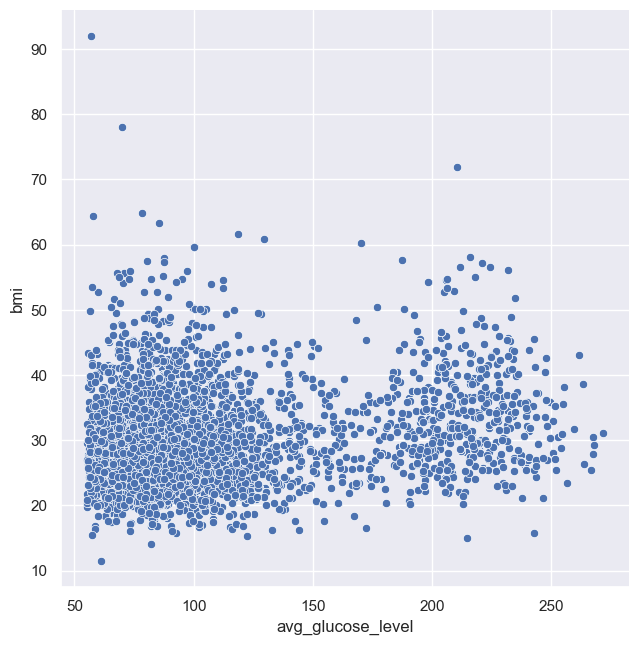
\includegraphics[width=0.8\textwidth]{bmi_glucose}
\end{figure}
